\chapter{渲染管线设计}
\section{渲染管线}

\subsection{多阶段屏幕空间折射}

实时折射如果完全按路径追踪计算，需要跟踪光线穿过薄膜前表面、后表面以及环境的多次传播，开销较大。项目采用 Wyman 的 image-space refraction 思路 \cite{wyman2005refraction}：先把可被折射的背景渲染成纹理，再在泡泡 shader 中根据法线和视线方向扰动采样坐标，从而得到近似折射效果。为了在鸿蒙端同时组织主泡泡、展示泡泡和前后景关系，系统在 Native 层采用多阶段 FBO 合成，但核心光学思路仍然是用两个屏幕空间界面近似肥皂泡的双界面折射。

\begin{figure}[H]
  \centering
  
\includegraphics[width=0.92\linewidth]{pipeline_pic2.jpeg}
  \caption{屏幕空间折射主线与多阶段 FBO 合成关系。}
  \label{fig:pipeline}
\end{figure}

这一主线被组织为以下几个连续阶段：

\begin{enumerate}
  \item \textbf{背景阶段}：将天空盒和背景参照物渲染到 \codepath{backgroundFBO}。
  \item \textbf{后景阶段}：把主泡泡后方场景写入 \codepath{sceneBehindFBO}，为背面折射提供输入。
  \item \textbf{背面阶段}：开启正面剔除，只绘制主泡泡背面，并输出到 \codepath{backFaceFBO}。
  \item \textbf{主场景阶段}：绘制包含交互泡泡的场景到 \codepath{mainSceneFBO}，供后续合成采样。
  \item \textbf{最终合成阶段}：将所有泡泡合成到 \codepath{finalSceneFBO}，再输出到屏幕。
\end{enumerate}

这种方法的优点是完全运行在 GPU rasterization 管线中，不需要逐像素射线求交；缺点是折射对象必须已经出现在屏幕空间纹理中，因此它是视觉上可信的近似，而不是严格物理光线追踪。对于鸿蒙终端场景而言，这种取舍能够在移动端预算下同时满足折射观感、多泡泡层次和交互响应速度。

\subsection{FBO 尺寸策略与坐标修正}

系统在 \codepath{InitFBO} 中采用低分辨率 FBO 合成，再由全屏四边形放大到最终屏幕，以兼顾移动端性能与画面完整性。其核心策略可写为：

\[
W_{\mathrm{fbo}} = 0.5 W_{\mathrm{screen}}, \qquad
H_{\mathrm{fbo}} = 0.5 H_{\mathrm{screen}}.
\]

由于 FBO 分辨率与窗口分辨率不同，正面渲染到屏幕时，\codepath{gl\_FragCoord} 是窗口像素坐标；背面渲染到 FBO 时，\codepath{gl\_FragCoord} 是 FBO 像素坐标。项目通过 \codepath{uRenderToFBO} 区分两种情况：

\begin{lstlisting}[language=C++]
vec2 fboPixel = (uRenderToFBO == 1)
    ? screenPixel
    : screenPixel * (uFBOSize / uWinResolution);
\end{lstlisting}

该修正对多泡泡渲染尤其重要。各泡泡在不同 pass 中复用同一套折射与虹彩 shader，如果输入坐标不能正确映射到 FBO 空间，就会出现采样越界或局部发黑。修正后，所有交互泡泡都沿用统一材质逻辑，并通过模型矩阵、局部几何扰动强度、虹彩模式、输出透明度以及是否响应交互等参数来区分。

\section{屏幕空间折射实现}

\subsection{折射方向}

在 fragment shader 中，入射方向取视线方向 \codepath{eye}，法线取世界法线 \codepath{normal}。肥皂液近似水的折射率，程序使用

\[
\eta = \frac{n_{\mathrm{air}}}{n_{\mathrm{film}}} = \frac{1.0}{1.33}.
\]

GLSL 中调用 \codepath{refract(eye, normal, eta)} 得到折射方向，并转换到视图空间：

\begin{lstlisting}[language=C++]
vec3 refractVec = mat3(vView) * refract(eye, normal, iorRatio);
\end{lstlisting}

随后取折射方向的 $xy$ 分量作为屏幕空间偏移方向。因为这是屏幕空间近似，shader 并不计算真实光线与后表面的三维交点，而是把折射方向转化为背景纹理采样偏移。

\subsection{边缘增强与薄膜厚度影响}

肥皂泡的中心通常接近透明，轮廓处视觉效果更明显。程序用

\[
e = 1 - |\mathbf{V}\cdot\mathbf{N}|
\]

表示边缘程度，其中 $\mathbf{V}$ 是视线方向，$\mathbf{N}$ 是表面法线。随后通过 \codepath{smoothstep} 得到更平滑的边缘曲线：

\[
e_{\mathrm{profile}} = \mathrm{smoothstep}(0.18, 0.92, e).
\]

折射偏移的核心形式可写为：

\[
\Delta \mathbf{p}
= \mathbf{T}_{xy}\,
s_{\mathrm{ref}}\,
s_{\mathrm{face}}\,
s_{\mathrm{film}}\,
r_{\mathrm{px}}\,
s_{\mathrm{edge}}\,
s_{\mathrm{touch}},
\]

其中 $\mathbf{T}_{xy}$ 是视图空间折射方向的屏幕分量，$s_{\mathrm{ref}}$ 是用户可调的 \codepath{uRefractionStrength}，$s_{\mathrm{face}}$ 区分正面和背面，$s_{\mathrm{film}}$ 由薄膜厚度和边缘程度共同决定，$r_{\mathrm{px}}$ 是泡泡屏幕半径，$s_{\mathrm{edge}}$ 是边缘增强。

背面 pass 使用更小的折射强度：

\[
s_{\mathrm{face}} =
\begin{cases}
0.16, & \text{背面 pass},\\
1.0, & \text{正面 pass}.
\end{cases}
\]

这样做可以避免双界面叠加时背景被过度扭曲。最终偏移还会被 \codepath{uMaxOffsetRatio} 限制在泡泡屏幕半径的一定比例内，防止采样跳变。

\reportfigure{2.2.jpg}{0.5}{0.26\textheight}{背景小球经过主泡泡后的折射扭曲效果}

\section{薄膜虹彩模型}

\subsection{薄膜干涉基础}

肥皂泡薄膜的厚度通常为数百纳米，和可见光波长处在同一数量级。光线在空气--薄膜界面与薄膜--空气界面发生反射，两个反射波之间产生光程差。对某一波长 $\lambda$，相位差可写为：

\[
\phi_\lambda =
\frac{4\pi n d \cos\theta_t}{\lambda},
\]

其中 $n$ 是薄膜折射率，$d$ 是薄膜厚度，$\theta_t$ 是薄膜内部折射角。不同波长的反射强度随 $\phi_\lambda$ 改变，因此 RGB 颜色会随厚度、视角和法线方向变化。

项目中所有虹彩模式都使用动态厚度 $d$ 与视角项 $|\mathbf{V}\cdot\mathbf{N}|$ 作为输入，但三种模式计算反射率的方式不同。

\subsection{Kim2012 模式：实时 RGB 波长采样}

程序界面中的 \textbf{Kim2012} 模式对应 \codepath{uIridescenceMode = 0}。它参考 Kim 与 Park 关于实时肥皂泡虹彩渲染的做法 \cite{kim2012soapbubble}，在 shader 中直接计算薄膜对 RGB 三个代表波长的反射率。实现文件为 \codepath{shader\_refraction.h} 中的：

\begin{itemize}
  \item \codepath{fresnelCoefficients}
  \item \codepath{interferencePhase}
  \item \codepath{thinFilmReflectance}
  \item \codepath{kim2012Iridescence}
\end{itemize}

对每个波长，程序先计算 s 偏振和 p 偏振的 Fresnel 振幅系数，再用相位差得到反射率近似：

\[
R_\lambda =
\frac{r_s^2(1-\cos\phi)}{1+r_s^4-2r_s^2\cos\phi}
+
\frac{r_p^2(1-\cos\phi)}{1+r_p^4-2r_p^2\cos\phi}.
\]

当前版本采样的三个代表波长为：

\[
\lambda_R=615\mathrm{nm},\quad
\lambda_G=535\mathrm{nm},\quad
\lambda_B=465\mathrm{nm}.
\]

该模式的优点是公式直接、易解释，能清楚体现薄膜厚度和相位差对颜色的影响；不足是只用三个波长代表完整可见光谱，边缘颜色可能更鲜艳，也更容易出现强烈的 RGB 分离。


\subsection{Belcour Airy 模式：多波长 Airy 反射近似}

\textbf{Belcour Airy} 模式对应 \codepath{uIridescenceMode = 2}，也是当前默认模式。它参考 Belcour 与 Barla 对薄膜虹彩和 Airy reflectance 的建模思想 \cite{belcour2017iridescence}，但本项目没有完整实现论文中的微表面解析预积分，而是在肥皂泡 shader 中实现了一个面向移动端实时展示的简化 Airy 反射模型。

对某一偏振方向，薄膜多次内反射的复振幅可写为：

\[
A_\lambda =
r_{12}
+
\frac{t_{12}r_{23}t_{21}e^{i\phi_\lambda}}
{1-r_{21}r_{23}e^{i\phi_\lambda}},
\qquad
R_\lambda = |A_\lambda|^2.
\]

程序分别计算 s、p 两个偏振方向，再取平均。随后在 \codepath{belcourAiryWeightedIridescence} 中采样多个波长：

\[
430, 470, 500, 535, 575, 615, 650 \mathrm{nm}.
\]

这些波长再乘以经验 RGB 权重得到最终颜色。相比 Kim2012 模式，Belcour Airy 模式的颜色更平滑，环境反射也会被薄膜反射率染色，因此更适合作为最终鸿蒙版本的默认外观。

\subsection{不同模式对比}

\begin{table}[H]
  \centering
  \caption{不同虹彩模式的区别}
  \label{tab:modes}
  \begin{tabular}{p{0.18\linewidth}p{0.25\linewidth}p{0.23\linewidth}p{0.23\linewidth}}
    \toprule
    模式 & 计算方式 & 优点 & 局限 \\
    \midrule
    Kim2012 & shader 中实时计算 RGB 三个代表波长的薄膜干涉反射率。 & 公式直观，便于说明相位差、Fresnel 系数和厚度的关系。 & 只采样三个波长，颜色可能偏强，光谱连续性有限。\\
    Belcour Airy & 使用 Airy 风格的多次内反射公式，并采样多个波长加权合成。 & 颜色过渡更平滑，边缘和环境反射更自然，是当前默认模式。 & 是项目级简化实现，不是完整 Belcour 微表面预积分模型。\\
    \bottomrule
  \end{tabular}
\end{table}

\begin{figure}[H]
  \centering
  \begin{minipage}[t]{0.32\linewidth}
    \centering
    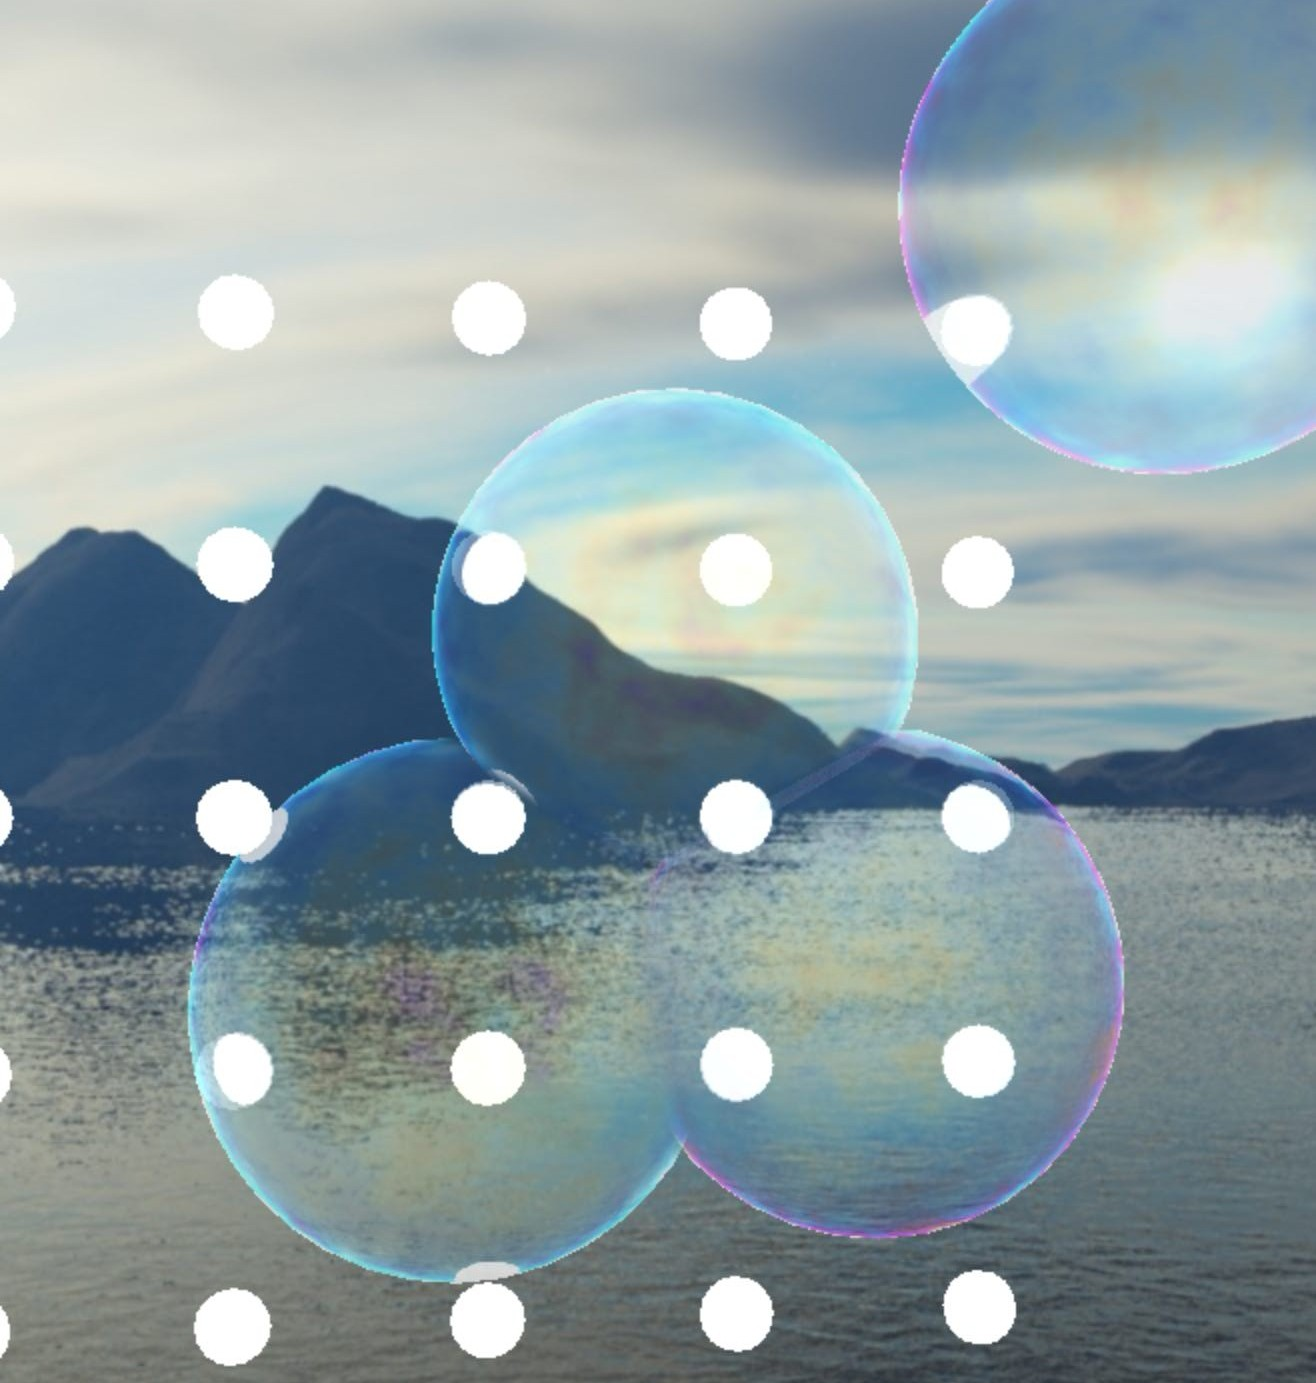
\includegraphics[width=\linewidth]{figures/2.3left.jpg}\\[0.4em]
    \small Kim2012
  \end{minipage}
  \begin{minipage}[t]{0.32\linewidth}
    \centering
    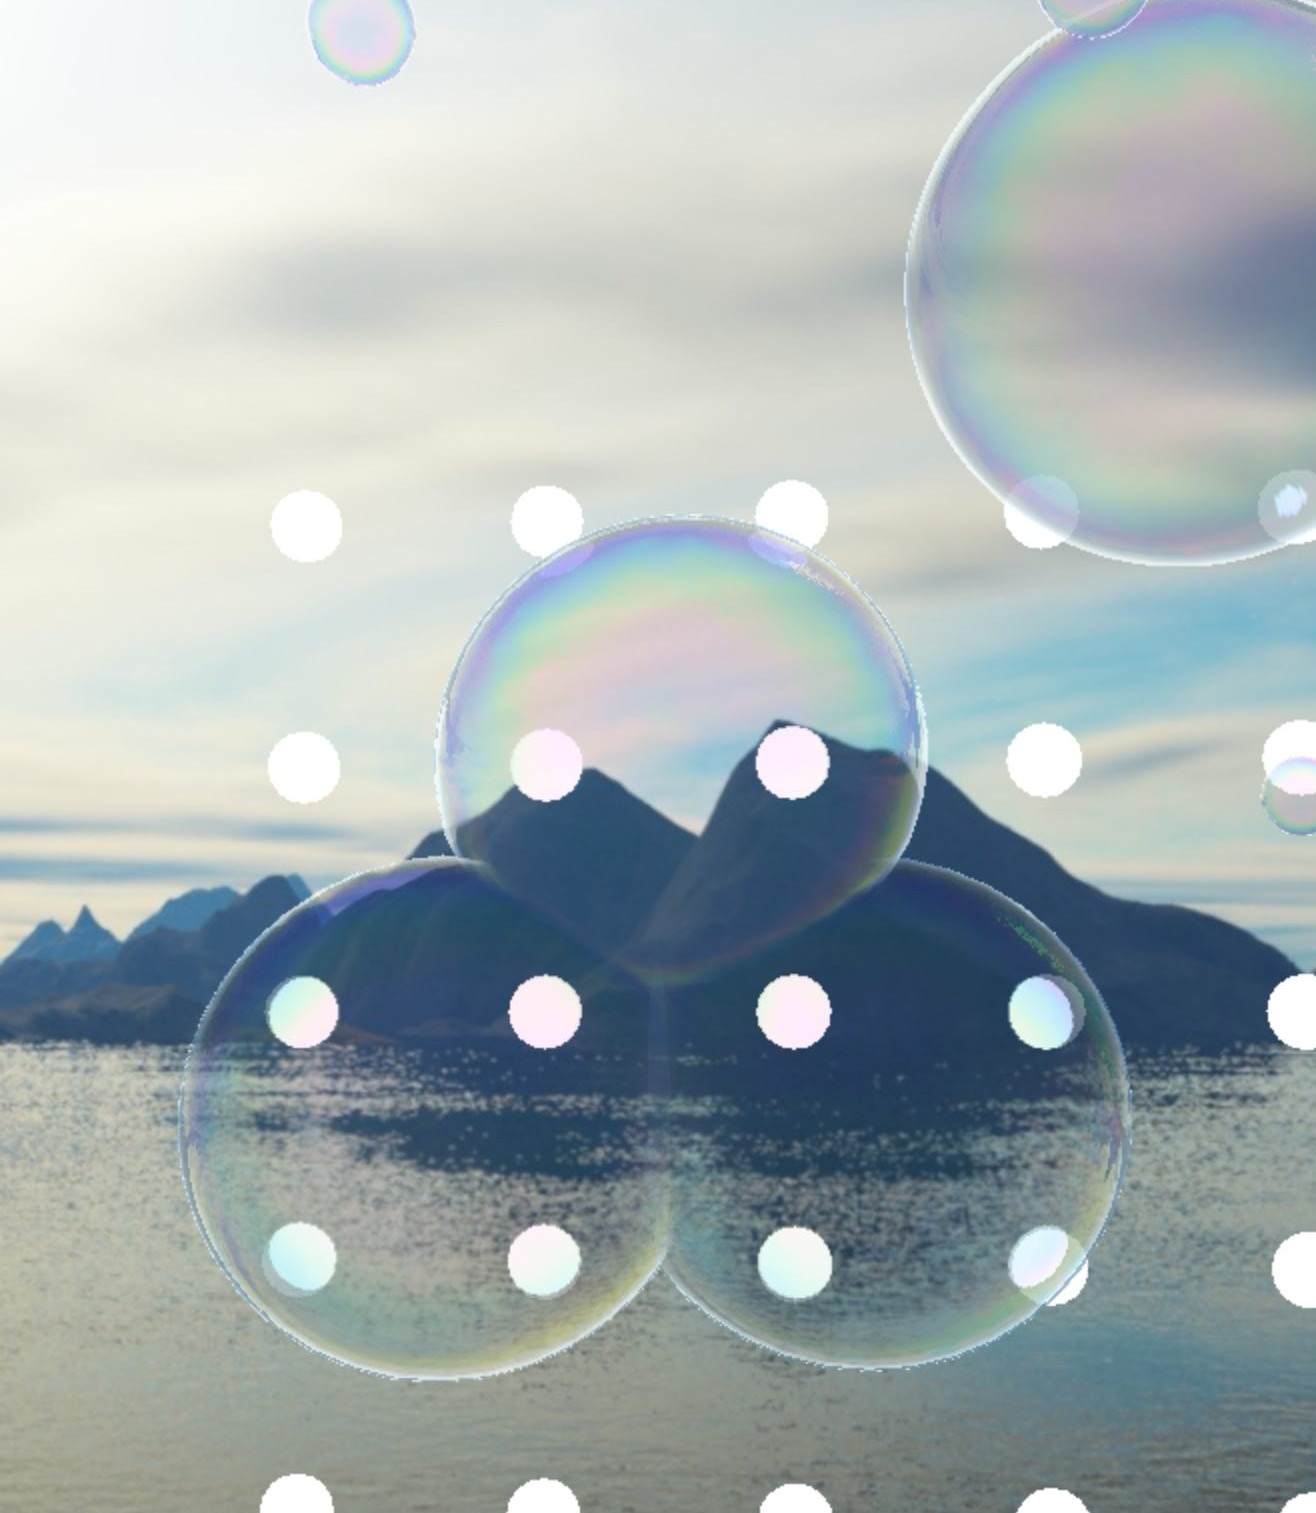
\includegraphics[width=\linewidth]{figures/2.3right.jpg}\\[0.4em]
    \small Belcour Airy
  \end{minipage}
  \caption{不同虹彩模式对比}
  \label{fig:three_modes}
\end{figure}

\section{动态膜厚与颜色合成}

\subsection{动态膜厚}

真实肥皂泡的膜厚会因为重力排液、表面流动和扰动而变化。完整的膜厚动力学可以基于表面上的流体方程建模 \cite{ishida2020thickness}。本项目为了满足移动端实时演示要求，采用 shader 中的程序化近似：使用世界法线方向作为膜面参数，叠加多层 Simplex noise、缓慢流动项、细节噪声和上下方向的排液趋势。

动态厚度可概括为：

\[
d =
d_0
+ A_{\mathrm{var}} P(\mathbf{n}, t)
+ 190 M_{\mathrm{touch}}
+ 95 Q_{\mathrm{ripple}},
\]

其中 $d_0$ 是基础膜厚，$A_{\mathrm{var}}$ 是膜厚变化幅度，$P(\mathbf{n},t)$ 是由多层噪声和排液项组合的厚度图案，其中 $d_0$ 是基础膜厚，$A_{\mathrm{var}}$ 是膜厚变化幅度，$P(\mathbf{n},t)$ 是由多层噪声和排液项组合的厚度图案。

一个重要实现细节是：项目使用 \codepath{normalize(vWorldNormal)} 作为噪声输入方向，而不是使用 UV 坐标。这样可以避免球体 UV 接缝处出现明显断裂，让虹彩流动更连续。

\subsection{颜色合成}

泡泡最终颜色由三部分组成：

\begin{enumerate}
  \item \textbf{透射背景}：从背景 FBO 或背面 FBO 中折射采样得到 \codepath{bgColor}。
  \item \textbf{薄膜虹彩}：由当前模式计算得到 \codepath{filmReflectance}，再根据 Fresnel 边缘项增强。
  \item \textbf{环境反射和高光}：通过 cubemap 采样环境反射，并用薄膜反射率染色；另外加入少量 Blinn-Phong 高光。
\end{enumerate}

中心区域透明度更高，轮廓处透明度下降、反射和虹彩增强。shader 中用

\[
F = (1 - |\mathbf{V}\cdot\mathbf{N}|)^{p}
\]

作为 Fresnel 边缘项，其中 $p$ 对应可调参数 \codepath{uFresnelPower}。这使泡泡中心能保持清透，边缘能呈现更明显的彩色轮廓。
